\documentclass{beamer}

\usepackage{fontspec}
\usepackage{polyglossia}
\setmainlanguage{russian}

\setmainfont{Times New Roman}
\setsansfont{Arial}
\setmonofont{Courier New}

\setbeamertemplate{footline}[frame number]

\title{Конструктор из геометрических примитивов}
\author{Студент: Семенчук М.А.\\
Руководитель: Шибанова Д.А.}
\institute{Факультет <<Информатика и системы управления>>\\
МГТУ им. Баумана}
\date{2026 г.}

\usepackage{graphicx}
\graphicspath{{images/}}

\begin{document}

\frame{\titlepage}

\begin{frame}{Цели и задачи}
    \textbf{Целью} данной работы является разработка ПО для визуализации трехмерных сцен, состоящих из геометрических примитивов, а также проведение исследования по оценке производительности разработанного ПО.

    \textbf{Задачи}:
    \begin{itemize}
        \item выбрать алгоритм генерации изображения, модель освещения и затенения;
        \item описать доступные для размещения на сцене модели и формализовать их;
        \item построить схемы алгоритмов;
        \item выбрать средства реализации;
        \item реализовать спроектированное ПО с помощью выбранных средств;
        \item провести исследование производительности разработанного ПО.
    \end{itemize}
\end{frame}

\begin{frame}{Трассировка лучей}
    Трассировка лучей --- метод рендеринга, который позволяет реалистично имитировать освещение среды за счет использования физически корректной модели поведения света.

    Распространяясь по сцене и взаимодействую с ее объектами, свет может рассеиваться, отражаться, поглощаться и преломляться.

    \begin{figure}[H]
        \centering
        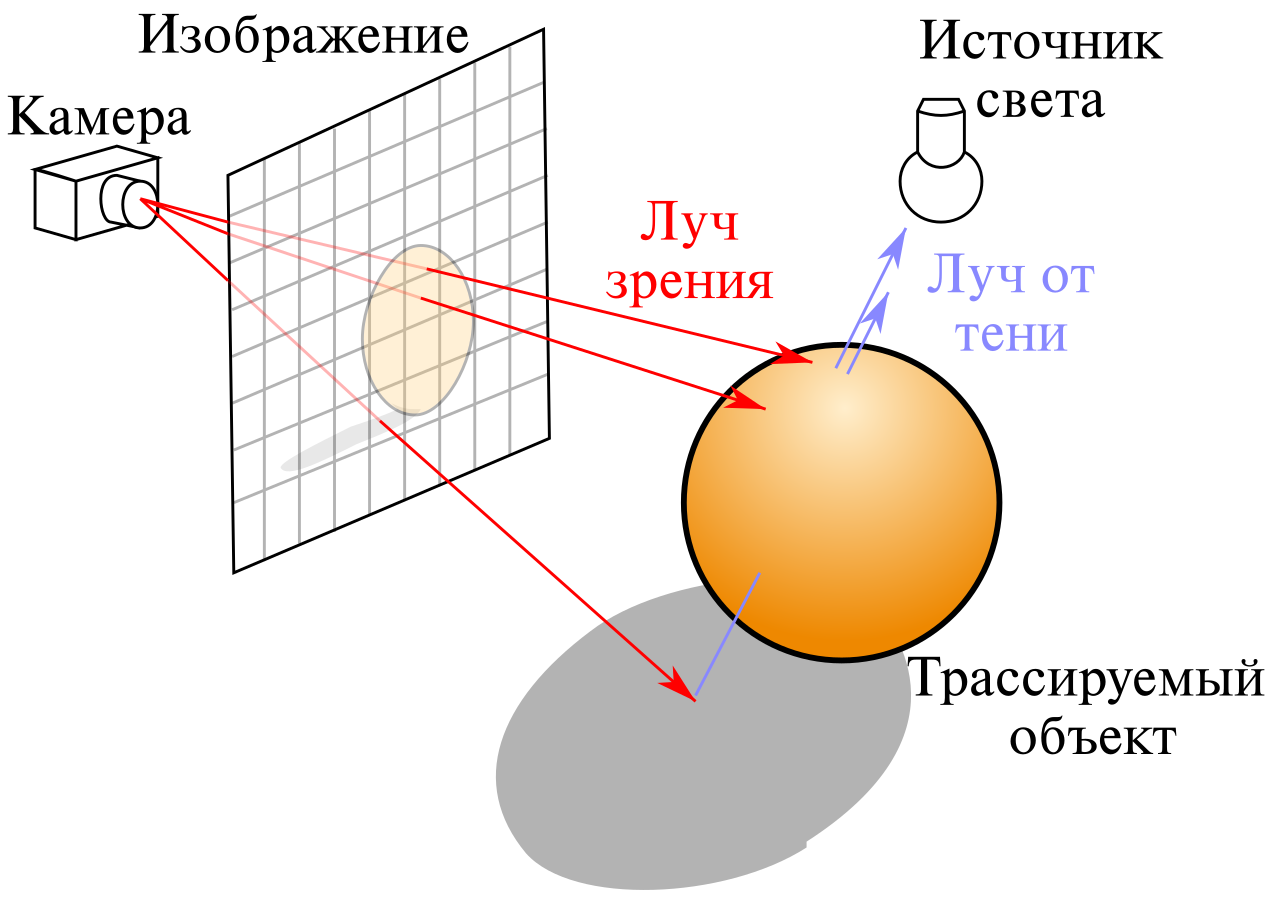
\includegraphics[width=0.35\textwidth]{ray_trace_diagram-ru.png}
        \caption{Диаграмма алгоритма обратной трассировки лучей}
    \end{figure}
\end{frame}

\begin{frame}{Модели освещения}
    \begin{figure}[H]
        \centering
        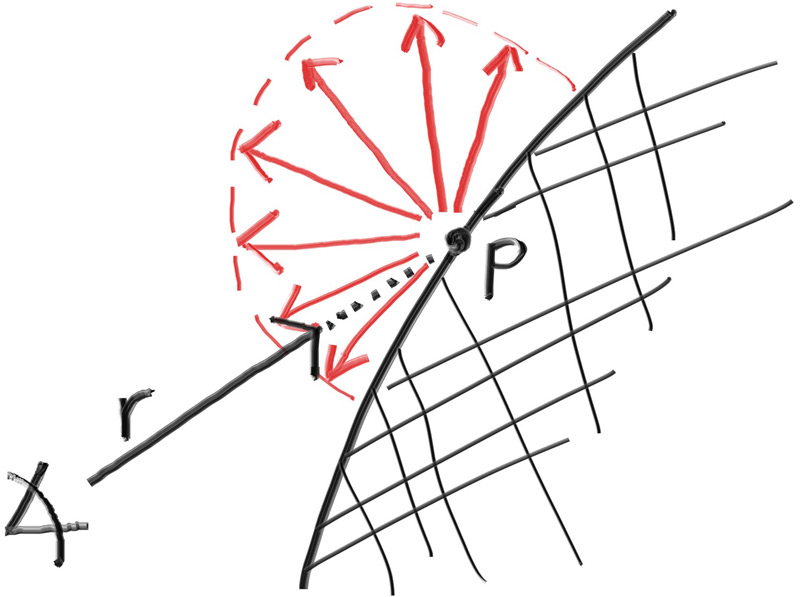
\includegraphics[width=0.35\textwidth]{diffuse_reflection.jpg}
        \caption{Модель освещения Ламберта (диффузное отражение)}
    \end{figure}

    \begin{figure}[H]
        \centering
        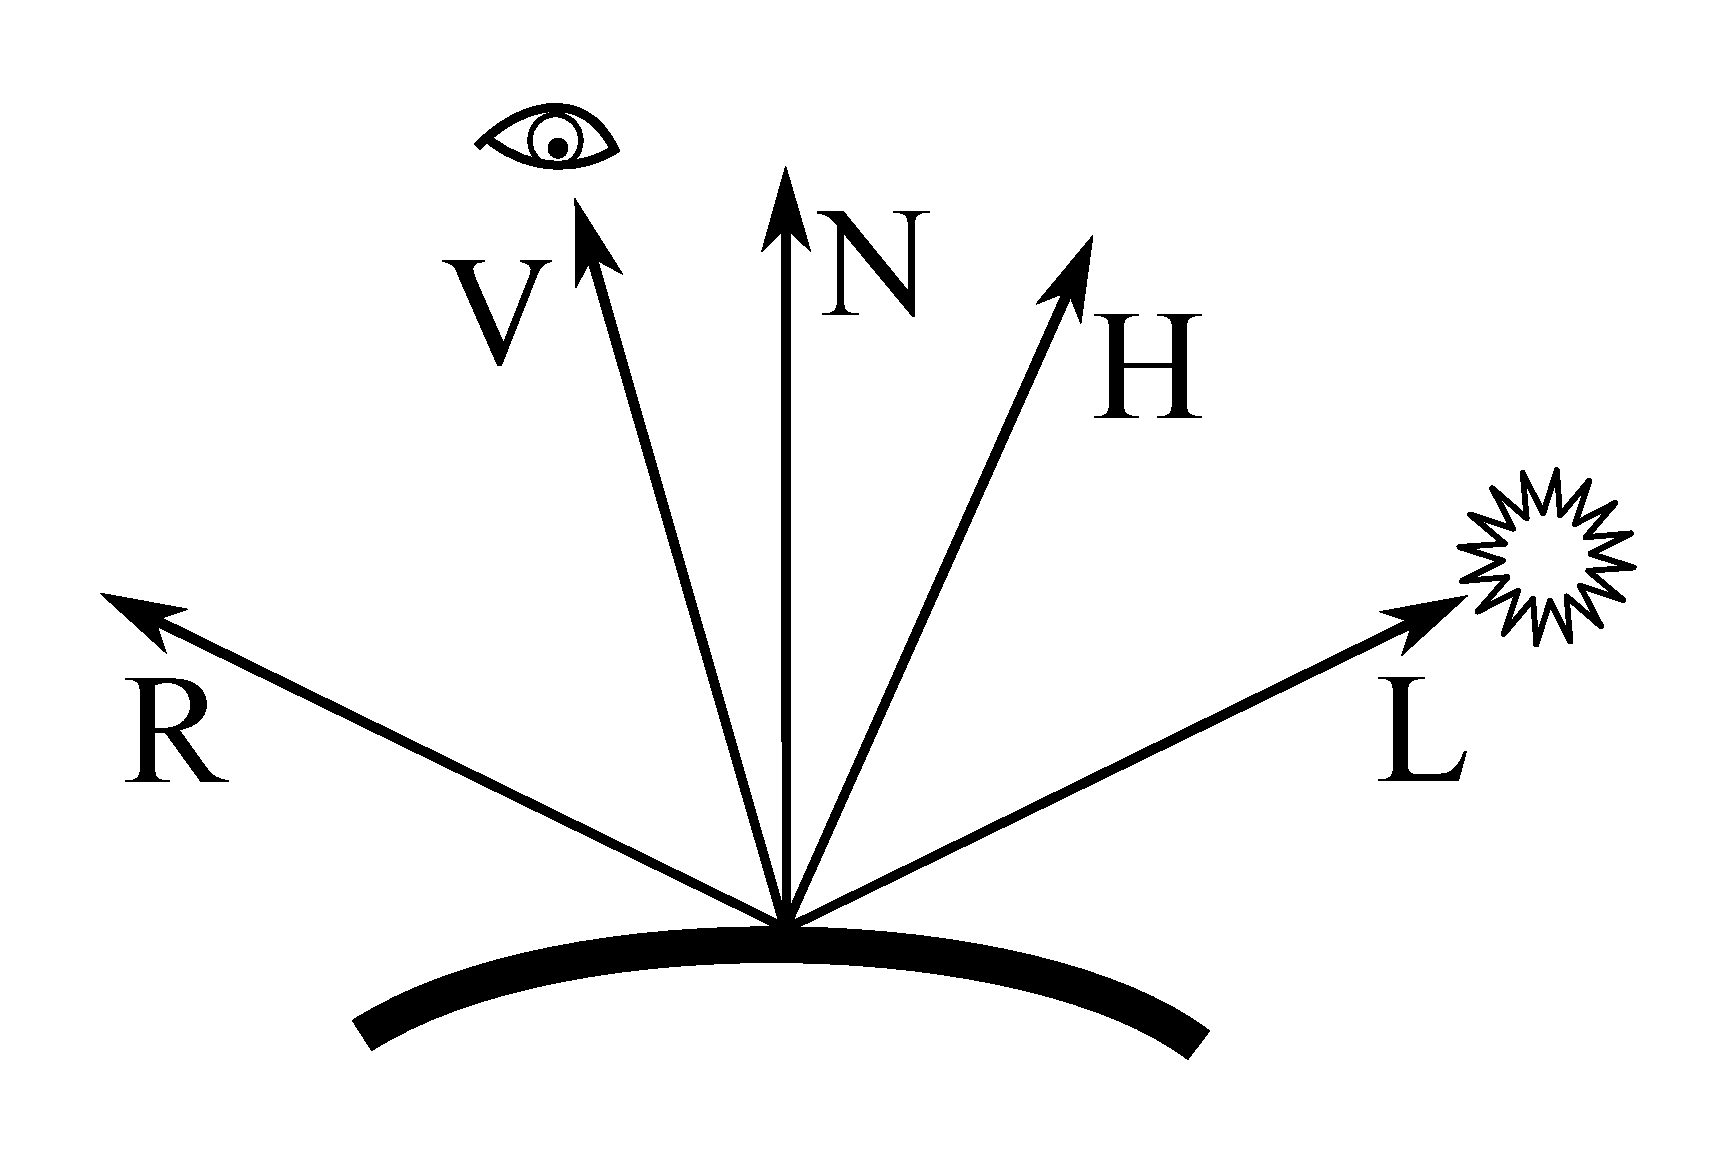
\includegraphics[width=0.35\textwidth]{blinn-phong_vectors.pdf}
        \caption{Диаграмма векторов модели Блинна-Фонга}
    \end{figure}

    \begin{figure}[H]
        \centering
        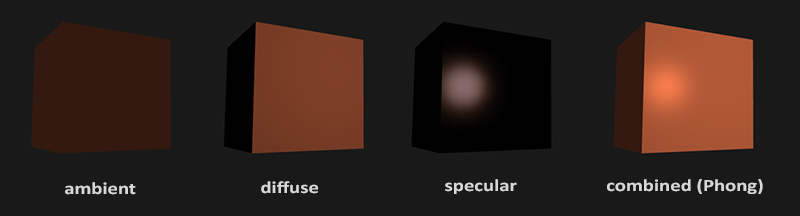
\includegraphics[width=0.65\textwidth]{phong_components.png}
        \caption{Компоненты модели освещения Фонга}
    \end{figure}
\end{frame}

\end{document}
